\chapter{The \LHC and \CMS detector} \label{chap:detector}

%\chapterquote{}{}

%------------------------------------------------------------------------------%
\section{Introduction}

% TODO: Careful of overlap with introduction chapter
The \LHC was built with the design goal of leading the energy frontier of high energy physics. This led to the successful discovery of the Higgs bosons by the \ATLAS \cite{Aad:1471031} and \CMS \cite{Chatrchyan:1471016} experiments.  Moreover, \BSM searches with these experiments continue to push stringent limits on the possible parameter-space of theorised new physics scenarios.  Such discoveries and searches are only possible by the hugely complex detectors and the \LHC accelerator complex, built and maintained by thousands of Engineers and Physicists.

%------------------------------------------------------------------------------%
\section{The \LHC}

\subsection{Accelerator Complex}

Proton collisions at the \LHC \cite{Bruning:782076} start from the ionisation of hydrogen gas to liberate the proton nuclei from their bound atomic states. Subsequently, the protons are accelerated by the radio-frequency (RF) cavity based accelerator \LINACTWO and injected into the \PSBooster\ --- four superimposed synchrotron rings accelerating protons from ${\SI{50}{MeV}}$ to ${\SI{1.4}{GeV}}$ --- to enhance the intensity of the proton injected into the \PS. The \PS is a synchrotron with a radius of ${\SI{72}{m}}$ bending the proton beam into a ring with energies up to ${\SI{25}{GeV}}$ before being injected into the \SPS.  Prior to this injection the proton beam is bunched into discrete packets of protons about ${\SI{4}{ns}}$ long with an equal spacing of ${\SI{25}{ns}}$ required by the \LHC for a bunch crossing rate of ${\SI{40}{MHz}}$. The \SPS is another synchrotron with a larger radius of ${\SI{6.9}{km}}$ to accommodate the acceleration of protons up to ${\SI{450}{GeV}}$ for the extraction by the \LHC. The whole accelerator complex, shown in Fig.~\ref{fig:LHC-Complex}, allows the \LHC to accelerate protons bunches up to energies of ${\SI{6.5}{TeV}}$ with a bunch crossing period of ${\SI{25}{ns}}$ and luminosities of the order of ${\SI{e34}{cm^{-2}s^{-1}}}$ \cite{Bruning:782076}.

\begin{figure}[htb]
    \centering
    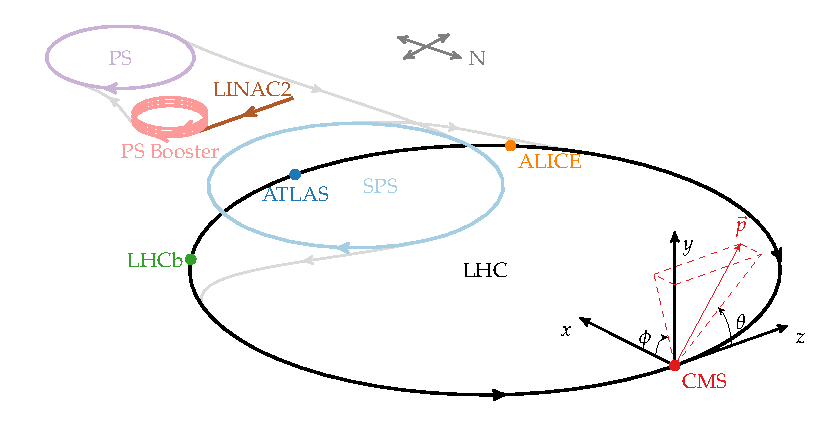
\includegraphics{diagrams/tikz/lhc_complex/lhc_complex.pdf}
    \caption[Schematic view of the LHC complex.]{
        An isometric schematic view of the \LHC complex chain delivering proton-proton collisions at the four main detectors: \LHCb, \ATLAS, \ALICE and \CMS. The coordinate system used by the \CMS detector is shown in both cartesian and polar coordinates. The pseudorapidity $\eta$, defined as $-\ln(\tan(\theta/2))$, typically replaces the $\theta$ angle because of its convenient properties under Lorentz transformations. This diagram is not to scale and the relative positions of the rings are guides to the physical positions.
    }
    \label{fig:LHC-Complex}
\end{figure}


\subsection{\LHC Main Ring}

The main physics goals of the \LHC project was the discovery of the Higgs boson, to observed new physics and rare \SM processes. The expected rate of a particular process with a cross section $\xs$ at an integrated beam luminosity $L$ is
%
\begin{equation}
    \mathcal{N} = L \xs \ .
\end{equation}
%
The event rate at the \LHC is directly controlled by the luminosity. For a Gaussian distributed beam, the luminosity can be given in terms of beam parameters as:
%
\begin{equation}
    \label{eq:beam-lumi}
    L = \frac{N_b^2 n_b\frev\relgamma}{4\pi\emitt\bstar} F\ ,
\end{equation}
%
where $N_b$ is the number of particles per bunch, $n_b$ is the number of bunches per beam, \frev is the revolution frequency, \relgamma is the relativistic gamma factor, \emitt is the normalised transverse beam emittance, \bstar is the beta function at the collision point (related to the transverse size of the beam) and $F$ is the geometric luminosity reduction factor due to the crossing angle of each beam at the crossing point.

At the \LHC, the luminosity is maximised by tuning all parameters in Eq.~\eqref{eq:beam-lumi}. This necessitated the use of proton beams circulating in separate vacuum chambers and merging at insertion points to the detectors. The beams nominally circulate in 2808 bunches with a spacing of ${\SI{25}{ns}}$ inside twin bore superconducting magnets --- two sets of coils and beam channels within the same structure and cryostat --- achieving a peak dipole field of ${\SI{8.33}{T}}$ to bend the beam. RF cavities apply the potential gradient to accelerate the protons from ${\SI{450}{GeV}}$ to ${\SI{6.5}{TeV}}$. Quadrupole magnets focus the beam to suppress dispersion to maintain the beam luminosity. Additional quadrupoles focus the beam as they enter the collision sections and defocus as they exit  \cite{Bruning:782076}.


\section{Compact Muon Solenoid (\CMS) Experiment}

The conditions provided by the \LHC during 2016 data taking resulted in an average number of collisions per bunch crossing of approximately 25, leading to 1000 charged particles every ${\SI{25}{ns}}$ bunch crossing. The \CMS detector \cite{Bayatian:922757} was designed to account for particle multiplicities of this order by focusing on high-granularity subdetectors with good time resolutions. This required a large number of detector channels and millions of synchronised detector electronics, all with a high radiation tolerance.

In addition to the conditions provided by the \LHC, the \CMS detector's design was driven by four main physics requirements to achieve a broad range of precision measurements and new physics searches, namely: searching for the Higgs Boson, supersymmetric particles, new massive vector bosons, extra dimensions; precision studies of the \SM; and heavy-ion physics. The physics requirements are summarised as follows:

\begin{enumerate}
    \item \textbf{Muon identification:} ability to clearly identify muons up to $\aeta=2.4$ and dimuon mass resolutions of about $1\%$ for transverse momenta of \SI{100}{GeV}, with an unambiguous charge up to momenta of \SI{1}{TeV}.
    \item \textbf{Charged particle reconstruction:} good momentum and reconstruction efficiency, particularly for the inner tracker, allowing for the identification of secondary vertices for the triggering and offline tagging of $\tau$'s and $b$-jets. This requires a tracker component with a few cm of the interaction point.
    \item \textbf{Electromagnetic energy resolution:} measure the diphoton and dielectron mass with a resolution of $1\%$ for transverse momenta of \SI{100}{GeV} up to $\aeta=2.4$. In addition, efficiently reject backgrounds from \Ppizero decays into two photons and maintain prompt lepton isolation at high luminosities.
    \item \textbf{Transverse missing momentum and dijet mass resolution:} near complete reconstruction of the proton interaction to measure the transverse missing momentum. This requires a hermetic detector with hadron calorimeters extending up to $\aeta=5.0$ and fine component segmentation in the $\eta$-$\phi$ plane of less than $0.1\times 0.1$.
\end{enumerate}

The full design of the \CMS detector is shown in Fig.~\ref{fig:cms-full} which achieves the requirements outlined above. The main distinguishing feature of the \CMS detector is a ${\SI{3.8}{T}}$ superconducting solenoid magnet enclosing the tracking and calorimetry subdetectors with an iron return yoke to maintain a ${\SI{2}{T}}$ field outside the solenoid for the muon subdetectors. All subdetectors are segmented into various regions in $\eta$ known as the barrel (covering the central $\eta$ range) and endcap (covering up to $\aeta=3.0$, with a slight overlap with the barrel). The hadronic calorimeter has an additional segment in the forward region, (covering $3<\aeta<5$) as required for the missing momentum reconstruction. Further subdetector dependent segmentation is done within the barrel, endcap and forward regions; discussed in further detail in the following subsections.  This gives the \CMS detector a total length of ${\SI{21.6}{m}}$ and a diameter of ${\SI{14.6}{m}}$ and weighing ${\SI{12500}{tons}}$.

\begin{figure}[htb]
    \centering
    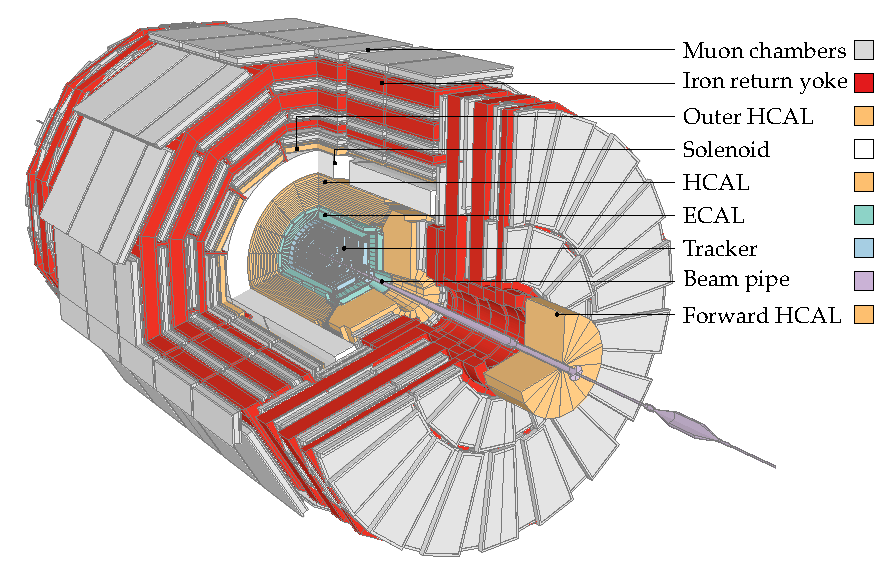
\includegraphics{diagrams/tikz/cms/annotated/cms_full.pdf}
    \caption[Schematic view of the CMS detector.]{
        A schematic view of the \CMS detector and subdetectors with a section removed to view the internal components. Acronyms are explained in the text. The diagram was produced using the tools outlined in \cite{Sakuma:2013jqa}.
    }
    \label{fig:cms-full}
\end{figure}

\subsection{Silicon Tracker}

The inner most subdetector, the silicon tracker \cite{Bayatian:922757}, measures the position of charged particles from ionisation deposits (known as hits) across a silicon-based reverse-biased p-n junction. A collection of hits is used to reconstruct the curved trajectory, with a radius of curvature $r$, of the particle with a charge $q$ within the magnetic field $B$ to determine the momentum of the particle transverse to the field, \pt, given by:
%
\begin{equation}
    \pt = rqB\ .
\end{equation}
%
A collection of tracks may intersect at a common point leading to the reconstruction of the primary interaction, pileup and secondary vertices.  All these vertices are typically a few centimetres apart, therefore, the tracker components are placed as near as ${\SI{4.4}{cm}}$ to the beam pipe.  The silicon tracker, shown in Fig.~\ref{fig:cms-tracker}, consists of two main components: pixels and strips. The pixels measure 3-dimensional positional coordinates of hits for environments of high particle flux (up to 10 million particles per second) near the beam. Pixel modules are arranged into three layers placed in the barrel region (BPIX) at radii of ${\SI{4.4}{cm}}$, ${\SI{7.3}{cm}}$ and ${\SI{10.2}{cm}}$ with a length of ${\SI{53}{cm}}$, centred on the z-axis. The pixel modules are staggered in the $\phi$-direction to achieve an overlapping configuration. Two additional pixel layers are placed in both endcap regions (FPIX) with a turbine-like geometry with the blades rotated by ${\SI{20}{\degree}}$ for overlapping blades. The overlap of pixel modules ensures the charged particle passes through at least one module in each layer. If two modules are hit the charge sharing between these modules provides additional positional information on the hit leading to improved position resolutions.

\begin{figure}[htb]
    \centering
    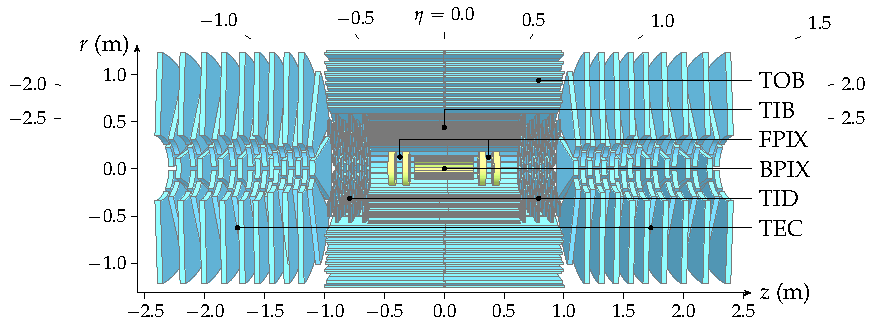
\includegraphics{diagrams/tikz/cms/annotated/cms_tracker.pdf}
    \caption[Cross-section view of the silicon tracker.]{
        A cross-sectional view, in the $y$-$z$ plane, of the silicon tracker.  The full tracker is shown in the upper part of the figure with a zoomed inset of the inner tracker in the central section and a further zoomed inset of the pixel tracker in the lowest part. The acronyms labelling various sub-components are defined in the text. The diagram was produced using the tools outlined in \cite{Sakuma:2013jqa}.
    }
    \label{fig:cms-tracker}
\end{figure}

Silicon strips are used further away from the beam pipe as the particle flux reduces. Strips provide an accurate 2-dimensional position for hits, hence layers are typically oriented in a stereo-configuration\footnote{A stereo-configuration has layers rotated at an angle with respect to each other to form a crosshatch pattern.} for the full 3-dimensional position. The silicon strips are separated into an inner and outer component. The inner component is further split by the barrel and endcap regions. The tracker inner barrel (TIB) component consists of four layers positioned at a radius of $20$--${\SI{55}{cm}}$ and covering ${|z|<\SI{65}{cm}}$ with cell sizes of ${\SI{10}{cm}\times\SI{80}{\micro m}}$. The first two layers use the stereo-configuration with an angle of ${\SI{100}{mrad}}$. The tracker outer barrel (TOB) component has six layers extending the coverage to ${|z|<\SI{124}{cm}}$ and ${\SI{55}{cm}<r<\SI{116}{cm}}$. Again the first two layers are placed in a stereo-configuration with an angle of ${\SI{100}{mrad}}$. The inner endcap (TID) component provides coverage for the gap between the TIB and TOB with three small disks oriented perpendicular to the $z$-axis to avoid excessive shallow track crossing angles. The first two disks have a stereo-configuration. The tracker outer endcap (TEC) consists of nine disks extending into ${\SI{124}{cm}<|z|<\SI{282}{cm}}$ with stereo-configuration for the first two  and the fifth disks \cite{Borrello:687861}. The entirety of the silicon detector consists of 66 million pixels and 9.6 million silicon strips with near hermetic coverage up to $\aeta=2.4$.

To process the data from the pixels and strips an on-detector chip processes and buffers the analogue signal while waiting on a decision to accept or reject the data (detailed in Sec.~\ref{sec:hardware-trigger}). Upon an accept signal being received the data is transmitted over optical links to off-detector chips for further processing, such as digitisation and data formatting.


\subsection{\ECAL}

The \ECAL \cite{Bayatian:922757} is a homogeneous calorimeter made of lead tungstate (\pbwo) crystals designed to measure electromagnetic deposits (typically electrons and photons) up to ${\aeta=3.0}$. The choice of lead tungstate scintillating crystals was driven by their short radiation lengths, $X_0$ (${\SI{0.89}{cm}}$), and Moliere radius\footnote{A radiation length is the distance travelled by a particle through a material where, on average, the particle has lost $63.2\%$ of it's original energy. Similarly, the Moliere radius is the radius of a cylinder which captures, on average, $90\%$ of the particle's shower, transverse to the initial direction of travel.} (${\SI{2.2}{cm}}$) with fast responses ($80\%$ of the light emitted is within ${\SI{25}{ns}}$) and have a satisfactory level of radiation resistance. These properties allow a compact design fully enclosed within the solenoid with sufficient containment of electron and photon showers both laterally and along the length of the crystals. The drawbacks of the crystal include low light yield (${\SI{30}{photon/MeV}}$) requiring a coupling to photodetectors with intrinsic gains operable in the magnetic field, and deterioration from continuous irradiation monitored throughout.

The \ECAL is divided into the barrel section (EB) and the two endcap sections enclosing the forward regions consisting of the endcap crystals (EE) and the preshower (ES), diagrammatically shown in Fig.~\ref{fig:cms-ecal}. The EB has an inner radius of ${\SI{129}{cm}}$ with the crystals titled at a ${\SI{3}{\degree}}$ angle in $\phi$ and $\eta$ with respect to the nominal vertex position to avoid particles travelling fully between two crystals. The crystals cover a $0.0174$ (${\SI{1}{\degree}}$) angle in $\phi$ and $\eta$ with the front face cross-section of ${22\times\SI{22}{mm^{2}}}$ and a length of ${\SI{230}{mm}}$ corresponding to $25.8X_0$. A submodule consists of 5 pairs of crystals held together by a thin-walled glass-fibre structure. The submodules are assembled into groups of 40--50 including the readout electronics and thermal screen.  Four modules are placed side-by-side to create a supermodule that covers half the length of the barrel and ${\SI{20}{\degree}}$ in $\phi$, two halves of 18 supermodules make the EB, covering a range of up to ${\aeta=1.479}$. The front face of the EE are placed at ${|z|=\SI{314}{cm}}$ from the nominal vertex and extends the \ECAL coverage in the range ${1.479<\aeta<3.0}$. Each endcap consists of two dees --- semi-circular aluminium plates with structural support units --- with crystals arranged in an $x$-$y$ grid of $5\times 5$ groups known as supercrystals. Partial supercrystals are placed on the inner and outer boundaries of the EE. Each EE crystal has a frontal cross-section of ${28.6\times\SI{28.6}{mm^{2}}}$ and a length of ${\SI{220}{mm}}$ (corresponding to $24.7X_0$). The ES is placed in front of the EE, covering the range $1.653<\aeta<2.6$, and consists of two planes of silicon strip detectors behind disks of lead absorbers at depths of $2X_0$ and $3X_0$, respectively. The purpose of the ES is to initiate the electron or photon showers with granular tracking to distinguish the individual photons from the decay of ${\Ppizero\ra\gamma\gamma}$ for rejection and to provide directional information on the electron or photon. A preshower placed in barrel was rejected in favour of accommodating a larger tracker.

\begin{figure}[htb]
    \centering
    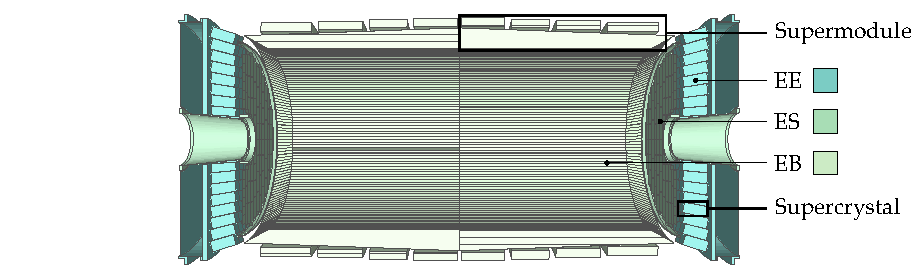
\includegraphics{diagrams/tikz/cms/annotated/cms_ecal.pdf}
    \caption[Front cross-section of the ECAL subdetector]{
        Front cross-sectional view of the \ECAL subdetector. Individual crystals are not shown, instead modules and supercrystals are displayed. The diagram was produced using the tools outlined in \cite{Sakuma:2013jqa}.
    }
    \label{fig:cms-ecal}
\end{figure}

The on-detector readout electronics for the \ECAL amplify and shape the signal from the photodiodes and digitise at the bunch crossing rate of ${\SI{40}{MHz}}$. This data is buffered until an accept signal is received to transfer the data to off-detector electronics for further processing. In addition to this processing, the on-detector electronics run fast algorithms on data from the ${5\times 5}$ clusters of crystals to aid in the accept decision, detailed in Sec.~\ref{sec:hardware-trigger}.

The energy of a shower determined from photodiode signals is corrected to reproduce the true energy of the particle initiating the shower. Several factors result in the need for a correction factor, namely: an imperfect clustering algorithm, energy loss from \brem, shower containment variations, imperfections within the crystals, crystal-to-crystal variations, misalignment of the crystals and limitations of the photodiodes. The reconstructed energy of a shower, $E$, is given by
%
\begin{equation}
    E = G\mathcal{F}\sum_i c_i A_i\ ,
\end{equation}
%
where $G$ is the global absolute scale in converting GeV, determined from in situ measurements of photons in ${\PZ\ra\mu\mu\gamma}$. The function $\mathcal{F}$ is a correction dependent on the type of particle; its position and momentum; and the clustering algorithm used, determined from simulation validated by test beam and in situ measurements of ${\PZ\ra ee}$ and ${\PZ\ra\mu\mu\gamma}$. The product of $c_i$ --- the intercalibration coefficients obtained from laboratory measurements, test beam precalibrations, comic ray measurements and in situ ${\PW\ra e\nu}$ measurements, and ${\Ppizero\ra\gamma\gamma}$ and ${\eta\ra\gamma\gamma}$ mass reconstruction --- and $A_i$, the signal amplitude, are summed over each clustered crystal labelled by $i$.

The corrected energy resolution of a supermodule is measured in a test beam by fitting a gaussian function to the reconstructed energy distributions and parameterised as
%
\begin{equation}
    \left(\frac{\sigma}{E}\right)^{2} = \left(\frac{S}{\sqrt{E}} \right)^{2}
    + \left( \frac{N}{E} \right)^{2} + C^2\ ,
\end{equation}
%
where $S=\SI{2.8}{\%}$ is a stochastic term, $N=\SI{12}{\%}$ is a noise term and $C=\SI{0.3}{\%}$ a constant term. The total energy resolution ranges between {$1.50$--$\SI{0.35}{\%}$} for {$10$--$\SI{250}{GeV}$}, beyond which the constant term dominates at $\SI{0.3}{\%}$ \cite{Chatrchyan:2008aa}.


\subsection{\HCAL}

The \HCAL \cite{Bayatian:922757} is designed to provide full coverage of hadronic activity from a proton-proton interaction, built from four distinct subdetectors, shown in Fig.~\ref{fig:cms-hcal} found in the barrel (HB), endcaps (HE), beyond the solenoid (HO) and far in the forward region (HF) \cite{Mans:1481837}. The HB and HE subdetectors are sampling calorimeters, fully immersed within the ${\SI{3.8}{T}}$ field, with a brass absorber and plastic scintillator tiles in a sampling ratio\footnote{The sampling ratio is the depth ratio of sampling to absorbing elements.} of about $3:40$. The HB and HE are separated by a gap at about $\SI{57}{\degree}$ designed to be non-projective with the interaction point to avoid particles traversing an uninstrumented gap.

\begin{figure}[htb]
    \centering
    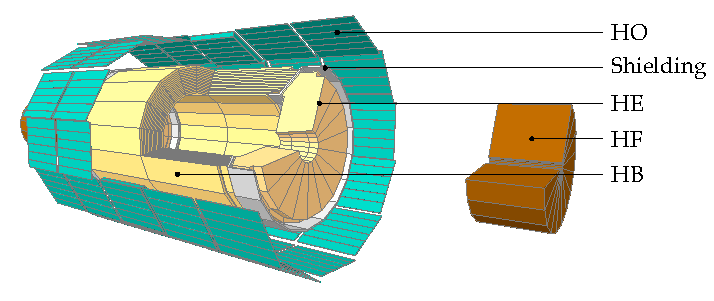
\includegraphics{diagrams/tikz/cms/annotated/cms_hcal.pdf}
    \caption[Front cross-section view of the four HCAL subdetectors]{
        Front cross-sectional view of the four \HCAL subdetectors. The magnet between the HB and HO, along with the other subdetectors have been omitted. The HF is placed beyond the muon endcaps extending the coverage of the \HCAL in the forward region. The diagram was produced using the tools outlined in \cite{Sakuma:2013jqa}.
    }
    \label{fig:cms-hcal}
\end{figure}

The HB covers the central region up to $\aeta=1.4$ with a inner radius of ${\SI{1777}{mm}}$ and outer radius of ${\SI{2876.5}{mm}}$, made of two half-barrels in $z$ of 18 identical wedges covering ${\SI{20}{\degree}}$ in $\phi$ with further segmented into  ${\SI{5}{\degree}}$ sectors. The wedges consist of towers: an alternating stack, parallel to the beam axis, of 17 active plastic scintillator tiles and brass plates, with the first and last absorber replaced by steel for structural strength, forming a tower.  Constraints on the space  between the \ECAL and solenoid restricted the HB to 5.7 hadronic interaction lengths at ${\eta=0}$ and up to 9 at ${\eta=1.4}$, necessitating the HO placed beyond the solenoid to improve the longitudinal containment of hadronic showers. Scintillation photons are produced from the interaction of hadronic showers with the active scintillation tile, collected by wavelength shifting (WLS) fibres embedded within the plastic spliced to clear fibres running along the tower. The optical signal is summed across the depth of a tower in three groups: the first, the next 4 and the final 12 scintillator tiles (${\{1+4+12\}}$). The clear fibres are coupled to by Silicon photomultiplers (SiPM). Full scintillator depth-segmentation would allow hadronic shower discrimination, however, the segmentation is limited by signal-to-noise, number of readout channels, power and cooling constraints.  Therefore, a balance of a three-depth configuration is in-place \cite{Mans:1481837}.

The HE subdetector in the endcap provides coverage in the region ${1.3<\aeta<3.0}$, overlapping the HB for improved coverage across the uninstrumented gap. The absorber-scintillator towers follow the same design as the HB towers with wedges covering ${\SI{20}{\degree}}$ in $\phi$, segmented to ${\SI{5}{\degree}}$ for towers in ${\aeta<1.74}$. The towers in ${\aeta>1.74}$ are instead segmented into ${\SI{10}{\degree}}$ to accommodate the bending radius of the WLS fibres. The $\eta$ segmentation also increases from ${0.087}$ for the towers at ${\aeta<1.74}$ to $0.09$--$0.35$ this $\eta$ range. The coarse azimuthal and polar segmentation allows for a finer depth segmentation with configurations of four or five-depths in-place, grouped by ${\{1+2+3+5+7\}}$. The HE provides sufficient material interaction lengths hence requires no outer calorimeter \cite{Mans:1481837}.

The HO consists of plastic scintillator tiles placed beyond the magnet to catch energy leakage from the HB. Instead of brass, the solenoid and iron return yoke act as the absorber extending the hadronic interaction lengths by $2$--$3$. Two scintillator layers are placed at ${\eta=0}$, either side of a ${\SI{19.5}{cm}}$ thick piece of iron, where the interaction length of the HB is the lowest. WLS fibres fed to SiPM detectors readout the signal from the HO. The segmentation follows that of the muon system with ${\SI{30}{\degree}}$ wedges divided into ${\SI{5}{\degree}}$ sectors in $\phi$ to overlap with the HB segmentation and five $\eta$ sectors up to ${\aeta=1.2}$. Partial plates are placed around the cryogenics and power cables for the magnet.

High intensity radiation falls upon the HF, placed at ${|z|=\SI{11.2}{m}}$ downstream of the interaction point. Consequently, an alternative design of steel absorbers embedded with radiation hard quartz fibres to produce \cherenkov radiation from hadronic showers, detected by multi-anode photomultiplier tubes \cite{Mans:1481837}. The steel absorbers are segmented in $\phi$ by ${\SI{20}{\degree}}$ wedges subdivided into two ${\SI{10}{\degree}}$ sectors, apart from the two towers nearest to the beam pipe which retain the ${\SI{20}{\degree}}$ segmentation. The steel absorber towers are placed parallel to the beam axis with an $\eta$ segmentation of approximately $0.175$, varying with $z$. The fibres also run parallel to the beam axis placed ${\SI{5}{mm}}$ apart in an $x$--$y$ grid with alternating long (full length of $10$ interaction lengths) and short (starting after $1.2$ interaction lengths). The two fibre lengths provide shower depth information similarly to the depth segmentation in the HB and HE \cite{Bayatian:2006jz}.

% Performance and calibrations?
%performance: Each subsystem has a laster and LED for monitoring and calibration. Since showers typically initiate in the ECAL the response and resolution of the CMS calo system depends on both the ECAL and HCAL. Corrections are determined from test beam studies. Resolution param by sigma/E = a/sqrt(E) oplus b. From test beams of earlier HCAL designs: a = stochastic term and b constant term. a=0.847 +- 0.016, b=0.074 +- 0.008 for EB. EE is similar. HF has a=1.98 and b=0.09.
%calibrations: absolute energy scale, detector response and uniformity. Test beam of e, pi and mu. These are monitored with in situ measurements.
%performance: pions and electrons over 5-300 GeV. Low energy performance studied with muons.


\subsection{Solenoid Magnet}

The muon identification requirement of the \CMS detector requires a large bending power provided by the solenoid magnet with a field strength of ${\SI{3.8}{T}}$. Such a high field is obtained by a superconducting magnet, shown in Fig.~\ref{fig:cms-magnet} maintained at operating temperatures by superfluid helium cooling. To extend the bending power the return field is focused by an iron return yoke spread throughout the muon chambers to about ${\SI{2}{T}}$.

\begin{figure}[htb]
    \centering
    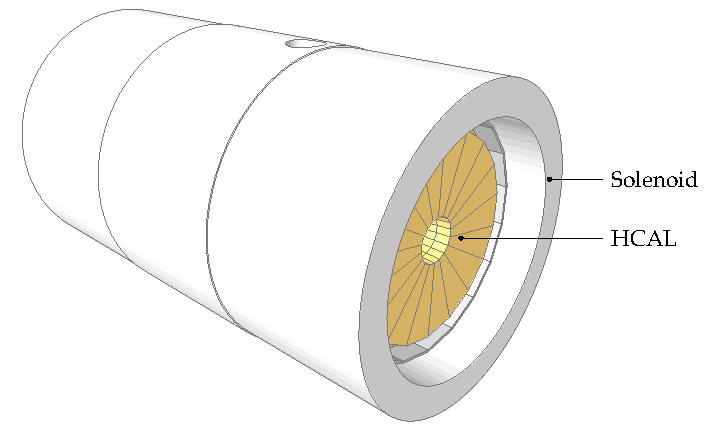
\includegraphics{diagrams/tikz/cms/annotated/cms_magnet.pdf}
    \caption[Isometric view of the CMS solenoid encompassing the HCAL.]{
        Isometric view of the solenoid and \HCAL with the muon chambers and HO removed. The diagram was produced using the tools outlined in \cite{Sakuma:2013jqa}.
    }
    \label{fig:cms-magnet}
\end{figure}


\subsection{Muon Chambers}

Muons from proton-proton collision, or secondary decays, travel through the detector leaving tracks in the tracker and energy deposits in the calorimetry system, however, most muons continue unscathed. The muon system \cite{Bayatian:922757} is designed to extend the 3-dimensional position measurements of these muons several metres away from the interaction point. Three types of gaseous detectors are used with the design driven by the large area to cover and different radiation environments, particularly between the barrel and endcap.

The layout of the three gaseous detectors in the \CMS muon system is shown in {Fig.~\ref{fig:cms-muon}}. In the barrel, anode wires centred in gas chambers, known as drift tubes (DT), collects the ionisation from passing charged particles for 2-dimensional position measurements. DTs perform poorly in the larger background and muon rate environment of the endcaps, hence cathode stripe chambers (CSC) are in-place. A charged particle ionises the atoms of the gas volume of a CSC with anode wires to collect the liberated electrons and perpendicular copper cathode strips where a mirror charge is induced allowing a full 3-dimensional position measurement. Resistive plate chambers (RPC) accompany both the DTs and CSCs to provide fast responses with good timing resolution at the cost of coarser positional resolution. The gas volume within an RPC is ionised by charged particles with the liberated electrons swept by an electric field induced from a large potential difference across plastic tiles either side of the gas volume. The electrons are collected by metal strips behind the plastic and the signal read out. The \CMS RPCs consist of a double-gap separating ${\SI{2}{mm}}$ thick bakelite tiles by a ${\SI{2}{mm}}$ gas gap.

\begin{figure}[htb]
    \centering
    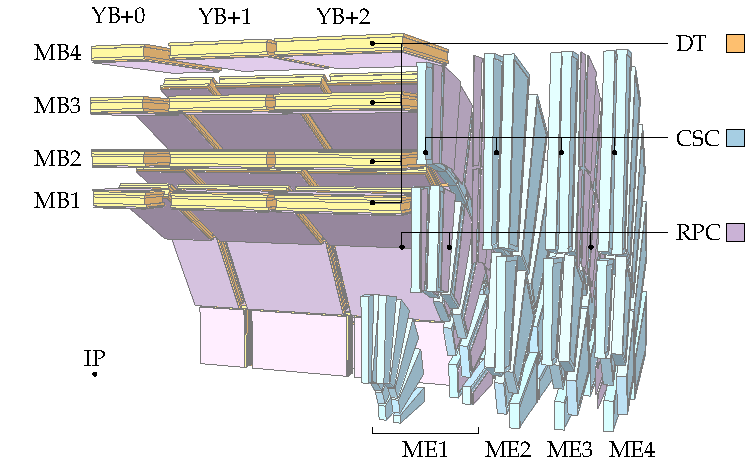
\includegraphics{diagrams/tikz/cms/annotated/cms_muon.pdf}
    \caption[Isometric view of an octant of the CMS muon systems.]{
        Isometric view of the rear-top-right octant of the muon system, omitting the iron return yoke. The interaction point (IP) is shown in the lower left. The division of the muon system into stations (MB), wheels (YB) and disks (ME) are discussed in the text. The diagram was produced using the tools outlined in \cite{Sakuma:2013jqa}.
    }
    \label{fig:cms-muon}
\end{figure}

The muon barrel section (MB) cover ${\aeta<1.2}$ and consists of four concentric stations labelled MB1--MB4 position at about $4.0$, $4.9$, $5.9$ and ${\SI{7.0}{m}}$ away from the beam axis. Each station is subdivided into 12 sectors in $\phi$, with subsequent sectors overlapping to avoid uninstrumented gaps. Two partial sectors are placed around the magnet cryogenic lines and power cables. The MB is divided into five wheels along $\eta$ labelled $\mathrm{YB}-2$ to $\mathrm{YB}+2$. Stations MB1 and MB2 consist of two RPCs placed either side of a DT chamber whereas MB3 and MB4 have one RPC placed on the inside of a DT chamber. These DT chambers consist of four layers of drift tubes, known as a superlayer (SL). Two SLs have their anode oriented along the beam axis to measure the $r$-$\phi$ coordinates of muon tracks, $\mathrm{SL}_{\phi}$, and the third SL rotated by ${\SI{90}{\degree}}$ measures the $z$ coordinate (omitted in MB4), $\mathrm{SL}_{\theta}$. The SLs are separated by a honeycomb (HC) structure in the order: $\mathrm{SL}_{\phi}$, HC, $\mathrm{SL}_{\theta}$, $\mathrm{SL}_{\phi}$; where the final $\mathrm{SL}_{\phi}$ is omitted in MB4.

The muon endcaps (ME) enclose the solenoid both ends of the \CMS detector with sufficient overlap with the barrel: $0.9<\aeta<2.4$. Both endcaps are divided into four disks, labelled ME1--ME4, perpendicular to the beam axis, subdivided into two concentric rings of 36 chambers (apart from ME2--ME4's innermost rings with 18 chambers each). The chambers within a disk overlap to avoid uninstrumented gaps. Each CSC is trapezoidal in shape with 6 gas gaps to measure the $z$ position, cathode strips projecting radially outwards  to measure the $\phi$ position and anode wires closely following the $\phi$ direction to measure the radial position from the beam axis. RPCs accompany each CSC up to $\aeta=2.1$.

%- Readout
%- Calibrations
%- Alignment

\subsection{Hardware Trigger}\label{sec:hardware-trigger}

The ${\SI{40}{MHz}}$ bunch crossing frequency provided by the \LHC at 2016 luminosities yields on average 25 proton-proton interactions per crossing leading to about 1 billion events per second. Storage capacities restrict full detector archiving of about 100 crossings per second. Therefore, an online\footnote{Online refers to tasks or processes performed in real-time with strict timing constraints whilst data taking. Conversely, offline refers to processing after the storage of data without strict timing constraints.} triggering system applies a rejection factor of the order of 1 in 10 thousand with minimal impact to the broad physics program. This system is realised in two-levels: the first level a hardware trigger (also known as the Level-1 trigger, \HWT) \cite{Bayatyan:706847,Tapper:1556311} with custom programmable processors, and a second level a software trigger \cite{Sphicas:2002gg} using general-purpose commercially available processors (discussed in Sec.~\ref{sec:software-trigger}).

The detector data for each bunch crossing is held in on-detector buffers whilst waiting on a decision from the \HWT to further process the crossing with the software trigger. The \HWT processes up to 128 bunch crossings simultaneously, allowing a total time of ${\SI{3.2}{\micro s}}$ on reaching a decision. The allocated time includes data transit time to the electronics, located in an adjacent cavern to the detector for radiation protection, which reduces the total processing time to about ${\SI{1}{\micro s}}$. The \HWT is sent a new bunch crossing to process every ${\SI{25}{ns}}$ and after the allocated time a decision must be made, also every ${\SI{25}{ns}}$. These restrictions prevent data fetching and result in most operations consisting of simple arithmetic or querying memory in lookup tables\footnote{A lookup table stores expensive computations in a pre-computed table for significant savings in processing time and complexity.}. Furthermore, information from the tracker and HO is omitted from the \HWT decision owing to their slow response. The other subdetectors provide coarse information, to reduce processing time, and are divided into the calorimeter and muon triggers with the candidates sent to the global trigger for the final decision.

The \HWT decision is based on reconstruction of individual objects such as photons, electrons, muons, jets, transverse energy sum or missing transverse energy (\etmiss). The physics requirements can be summarised, with examples of targeted physics, as follows:

\begin{enumerate}
    \item Triggering of events with a single lepton of ${\aeta<2.4}$ and ${\pt>\SI{40}{GeV}}$ with an efficiency above $95\%$ to target events with \PW decays.
    \item Dilepton triggers with the same kinematical requirements and an efficiency above $95\%$ to collect \PZ decays.
    \item Single photon and diphoton triggers with similar thresholds for processes involving a Higgs boson.
    \item \etmiss threshold about ${\SI{100}{GeV}}$ for sensitivity to new weakly interacting particles.
\end{enumerate}


\subsubsection{Calorimeter trigger}

\ECAL (EB and EE) and \HCAL (HB, HE and HF) signals are clustered into trigger towers: ${5\times 5}$ arrays of crystals in the EB and EE; single physical tower for the HE and HB up to ${\aeta=1.74}$ and twice the number of physical towers in $\phi$ beyond this, whereby the energy of the physical tower is divided equally between the trigger towers; and physical towers grouped into pairs in $\phi$ and threes in $\eta$ for the HF. The transverse energy of each trigger tower is determined by on-detector electronics and the result is sent to the \HWT electronics along with flexible pass-fail information to, for example, encode depth structure. This information is further processed with each bunch crossing sent to one of ten processing nodes (with two redundant nodes) to scan across the full ${\eta}$--${\phi}$ plane and identify physics objects: jets, $\tau$s, electrons and photons; as well as calculating the transverse energy sum and \etmiss. The processing nodes run concurrently with a new bunch crossing occupying the first node upon completion of the previous crossing. This is known as a time multiplexed system where the output must be reassembled into the original bunch crossing order (de-multiplexed) for the global trigger.


\subsubsection{Muon trigger}

The muon trigger system primarily consists of track finding from successive chamber hits by a muon. This is divided into regional track finders using a combination of the DTs and RPCs in the barrel (up to ${\aeta=0.8}$), CSCs and DTs in the endcaps (from ${\aeta=1.25}$) and all three chambers in the overlap region between the barrel and endcaps. Additionally, the system is tasked with assigning hits to the correct bunch crossing, achieved by the high timing precision of the RPCs and of the CSC's anode wire response. Timing is also performed with the DTs, albeit with a poor resolution due to long drift times of ${\SI{400}{ns}}$. The tracks from these regional triggers is sent to the global muon trigger to merge and remove duplicate muon candidates, along with combining the isolation information from the calorimeter trigger, and finally sorts the muons for the global trigger.


\subsubsection{Global trigger}

The trigger objects and variables received from the calorimeter and muon triggers is collected at the global trigger for synchronisation and correlation of relevant trigger candidates. The union of a set of requirements on the trigger objects is determined and forms the basis of the \HWT decision.  However, evolving conditions and the collection of events from high cross-sectional processes requires the global trigger to reject random events to reduce the trigger rate. This process is known as prescaling and reduces the trigger efficiency by the prescale factor: e.g. a prescale factor of 10 will accept 1 out of 10 events regardless of decision formed from the trigger candidates resulting in a rate reduction of a factor of 10 and a drop efficiency of $90\%$. After the prescaling is applied the \HWT decision is communicated to the data buffers to discard or transmit the bunch crossing to the software trigger.


\subsection{Software Trigger}\label{sec:software-trigger}

The software trigger (also known as the high-level trigger, \SWT) accepts the full detector granularity and all subdetector information from the on-detector readout. All bunch crossings filtered by the \HWT are distributed among processing nodes in a processor farm, each node running a copy of the software code to reconstruct and reject events. To meet the timing constraint, the \SWT performs a partial reconstruction of the event at first, guided by the trigger objects from the \HWT, gradually performing the full reconstruction until the event fails the trigger criteria. Furthermore, the \SWT must be efficient at selecting physics objects of interest and inclusive to avoid rejecting exotic physics. Therefore, the \SWT reconstruction is closely aligned with offline reconstruction (discussed in Chap.~\ref{chap:reconstruction}). However, calibrations and other run conditions available for offline analysis cannot be used. After accepting an event, the data is archived and made readily available for further analysis by the computing grid.


\subsection{Worldwide \LHC Computing Grid (\WLCG)}

Despite the data reduction achieved by the \CMS trigger system, a vast amount of data was accepted and requires prompt full reconstruction with possible revisions in light of improved object reconstruction, calibrations or code errors. Moreover, simulations of proton-proton collisions within the \SM and possible \BSM physics, including a simulation of the detector, the trigger and pileup with full reconstruction demands a significant amount of processing power. To achieve this the \WLCG was established \cite{Bird:1695401}. The \WLCG is a highly distributed computing cluster divided into tiers situated at: the main \CERN site, national laboratories and Universities worldwide. The computing  provides the resources required for data reconstruction and simulations, and supports in the design, evaluation, construction and calibration of the detector and future upgrades.


\section{Summary}

The \LHC provides proton-proton bunch crossings at a rate of ${\SI{40}{MHz}}$, a centre-of-mass energy of ${\SI{13}{TeV}}$, and the \CMS detector centred on one of these crossings. The \CMS detector is designed to detect and reconstruct the position and momenta of outgoing particles from the collisions whilst mitigating backgrounds such as noise and pileup, and optimising the geometry and readout channels with modern technology. The main feature is a ${\SI{3.8}{T}}$ solenoid enclosing the silicon tracker and calorimetry with an outer muon system. A two-level trigger system reduces the data output by selecting events of interest for a manageable output rate for archiving.  The immense processing power required for further analysis of the data and production of simulations is mediated by the \WLCG.
